\documentclass[border=8pt,12pt]{standalone}
\usepackage{times}
\usepackage{amsmath,amssymb,graphicx,xcolor}
\usepackage{tikz}
\newcommand{\g}[1]{\textcolor{black!55}{#1}}
\begin{document}
\begin{tikzpicture}
\node[anchor=west, inner sep=0pt] (defs) at (0,0) {%
\renewcommand{\arraystretch}{1.5}%
\begin{tabular}{@{}l@{}}
$E_{\rightarrow} = P(x \text{ entails } x')$ \\
$E_{\leftarrow} = P(x' \text{ entails } x)$ \\
$C_{\rightarrow} = P(x \text{ contradicts } x')$ \\
$C_{\leftarrow} = P(x' \text{ contradicts } x)$ \\[8pt]
$E_{\min} = \min(E_{\rightarrow}, E_{\leftarrow})$ \\
$C_{\max} = \max(C_{\rightarrow}, C_{\leftarrow})$ \\[8pt]
\textbf{Drift}: the shaded leaves
\end{tabular}};
\node[anchor=west, inner sep=0pt] at ([xshift=0.9cm]defs.east) {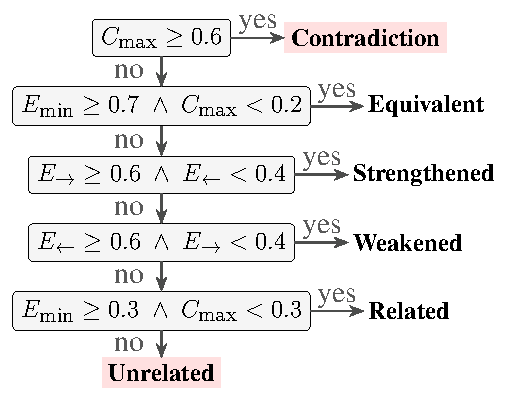
\includegraphics{nli-tree.pdf}};
\end{tikzpicture}
\end{document}
